13. $\cfrac{(x+1)(x+2)}{x^2+7x+12}\leqslant1 \Leftrightarrow \cfrac{x^2+2x+x+2-x^2-7x-12}{x^2+7x+12}\leqslant0 \Leftrightarrow
\cfrac{-4\left(x+\cfrac{5}{2}\right)}{(x+4)(x+3)}\leqslant0.$ Применив метод интервалов, найдём ответ: $x\in(-4;-3)\cup\left[-\cfrac{5}{2};+\infty\right)$
\begin{figure}[ht!]
\center{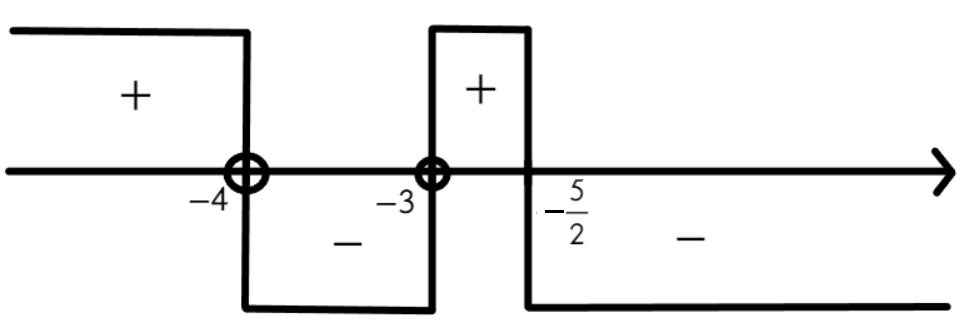
\includegraphics[scale=0.35]{ner9-13.png}}
\end{figure}\\
